\section{Problem Definition}
\label{probelm_def}
\subsection{Terminology}
An itemset is a set of items, written as \( i_{j_1}\ i_{j_2}\ \dots\ i_{j_k} \). The length of an itemset refers to the number of items it contains. A transaction is defined as a pair \((ts, X)\), where \(ts\) is a timestamp (an integer representing the time of occurrence) and \(X\) is an itemset. A list of transactions is called transaction data, denoted by \(D = [d_1, \dots, d_N]\). The length of the transaction data is the number of transactions it contains. In this study, we focus on data in which timestamps are recorded at fixed intervals.

We arrange the timestamps of each transaction in ascending order to form a list without duplicates,\(T = [ts_1, \dots, ts_N].\)
In this paper, a \emph{gap} denotes the distance between two successive occurrences of the same itemset in \(T\): if \(P\) appears at positions \(p_k\) and \(p_{k+1}\), then $  \mathit{gap} \;=\; p_{k+1} - p_k,$
which may exceed one when those occurrences are not adjacent. An \emph{interval}, by contrast, is the contiguous span defined by its start and end timestamps \([ts_i, ts_j]\) (with \(1 \le i \le j \le N\)), whose length is \(j - i + 1\). We denote by $D_I = [X_{ts_i}, \dots, X_{ts_j}]$ the list of itemsets corresponding to all transactions within this interval, and write its length as $n(D_I)$.

To identify itemsets that are dense within specific intervals, we use the interval support proposed by \cite{mahanta2005finding} as a measure of local occurrence frequency. Specifically, for an interval \(I = [ts_i, ts_j]\), the interval support of an itemset \(P\), denoted by \(Sup_I(P)\), is defined by Equation (\ref{eq:support}):

\begin{IEEEeqnarray}{rCl}
Sup_I(P)
= \frac{n\bigl(\{\,X\in D_I \mid P\subseteq X\,\}\bigr)}{n(D_I)}
\label{eq:support}
\end{IEEEeqnarray}
where \(D_I\) and \(n(\cdot)\) are as defined above.

In contrast to the support defined in frequent itemset mining \cite{agrawal1994fast}, which is normalized by the total length of the dataset, the interval support is normalized by the length of each interval \(I\) and thus measures the local frequency. Given thresholds \(minSup\) (minimum interval support) and \(minL\) (minimum interval length), we call an interval \(I = [ts_i, ts_j]\) a dense interval for an itemset \(P\) if it satisfies:

\begin{enumerate}
    \item \(Sup_I(P) \ge \textit{minSup}\), and  
    \item \((j - i + 1) \ge \textit{minL}\).
\end{enumerate}

% When listing dense intervals in ascending order of their timestamps, we denote the \(k\)-th such dense interval for \(P\) by \(CI_k^P\). 
If an itemset \(P\) has at least one dense interval, then \(P\) is called a dense pattern. Intuitively, \(\textit{minSup}\) determines whether the pattern appears sufficiently often in a given interval, while \(\textit{minL}\) enforces a minimum duration. A low \(\textit{minL}\) makes the method sensitive to brief bursts, whereas a high \(\textit{minL}\) smooths out short fluctuations and captures longer trends.

\subsection{Preliminary Experiments:Performance Issues}


\begin{figure}[t]
    \centering
    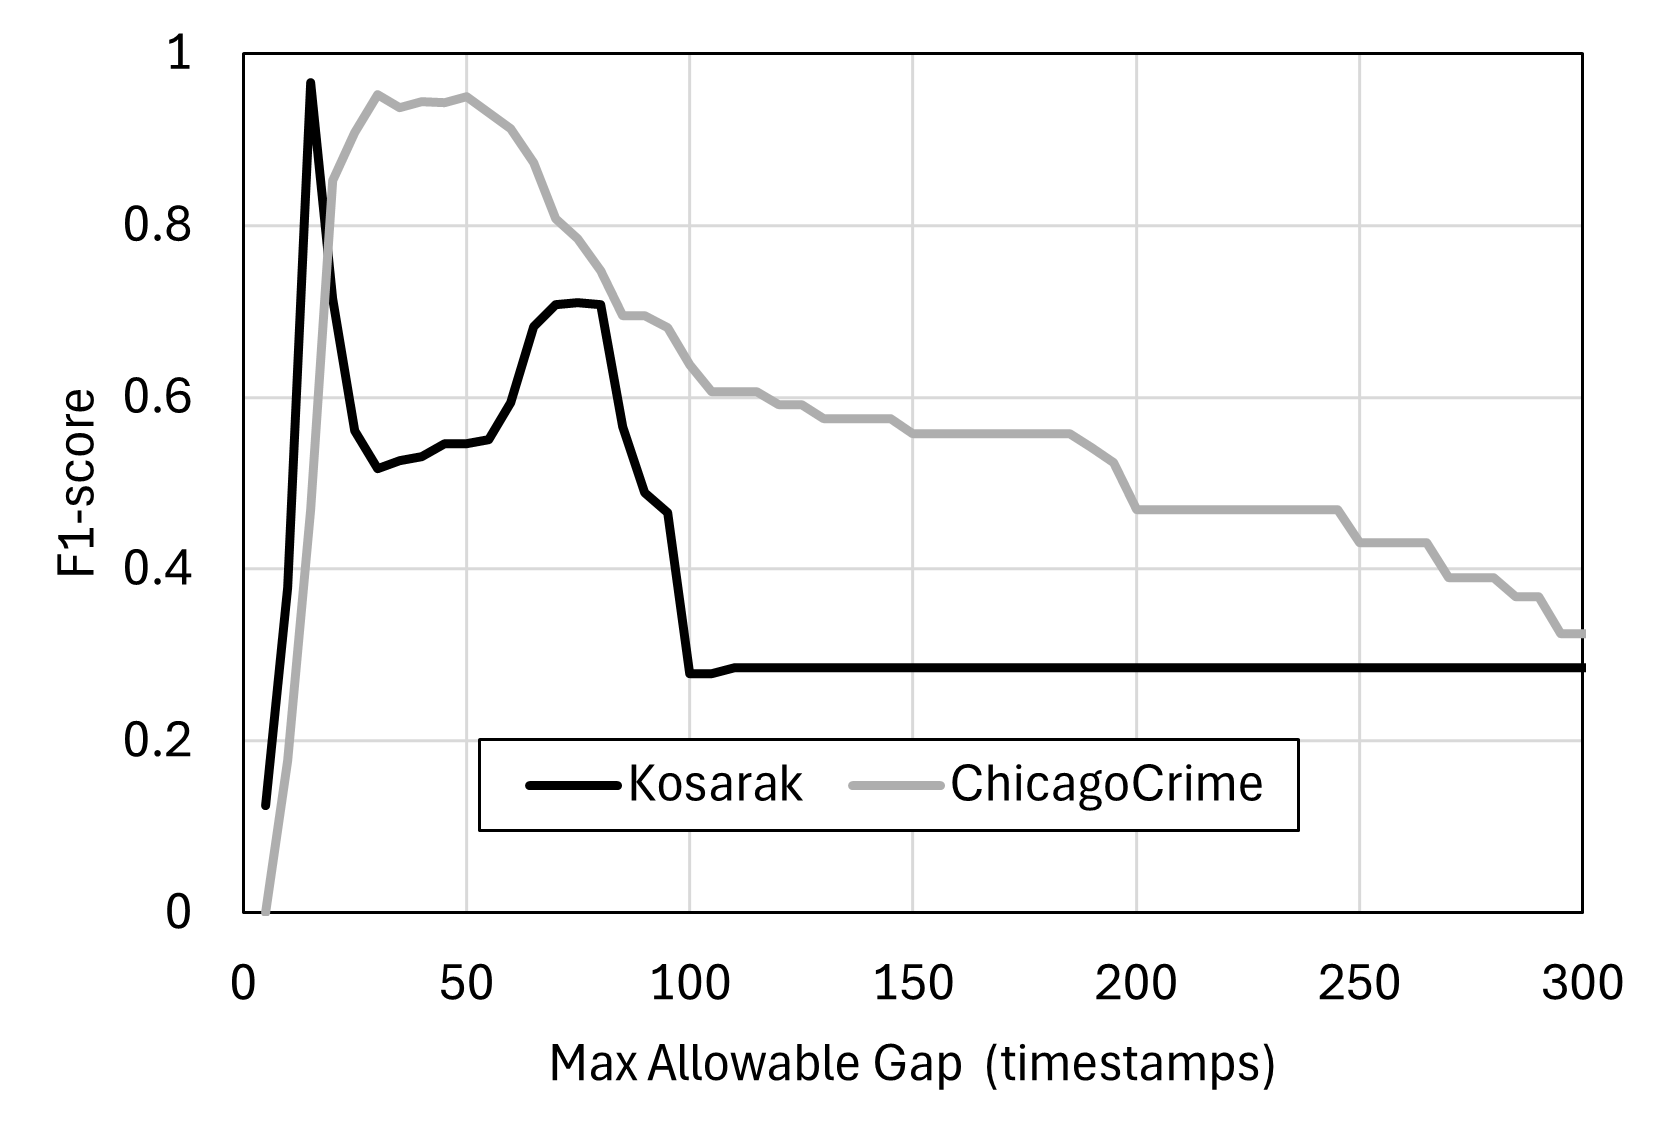
\includegraphics[width=1\linewidth]{fig/preliminary.png}
    \caption{Variation of extraction accuracy according to the maximum allowable gap when LPFIM is applied to extract dense patterns.The x-axis is the max allowable gap and the y-axis is the F1-score. This line indicates that the threshold setting of the max allowable gap affects the accuracy of the pattern detection.}
    \label{fig:acc_of_related_works}
\end{figure}

We conducted preliminary experiments to clarify the issues that arise when applying LPFIM\cite{mahanta2005finding} to the dense pattern extraction task. In these experiments, LPFIM was applied to two real-world datasets while the maximum allowable gap—a key parameter—was varied in increments of 5, and the resulting F1-scores were measured. Statistical details of the datasets are provided in Section \ref{sec:experiments}.

The target dense patterns were predetermined as ground truth. In the comparison between the ground truth and the itemsets extracted by LPFIM, we define recall as the fraction of ground-truth patterns covered by the extracted itemsets, precision as the fraction of extracted itemsets that correspond to true dense patterns, and compute the F1-score based on these two metrics (see Equations (\ref{eq:recall}), (\ref{eq:precision}) and (\ref{eq:f1score}) below).

\begin{IEEEeqnarray}{rCl}
Recall & = & \frac{\lvert A\cap G\rvert}{\lvert G\rvert}\,, 
\label{eq:recall}\\
Precision & = & \frac{\lvert A\cap G\rvert}{\lvert A\rvert}\,, 
\label{eq:precision}\\
F1\text{-}score & = & \frac{2\,\lvert A\cap G\rvert}{\lvert G\rvert + \lvert A\rvert}\,. 
\label{eq:f1score}
\end{IEEEeqnarray}


% For the preliminary experiments, the parameter settings were as follows: for the Kosarak, and ChicagoCrime datasets, the minimum interval length was 250 with a minimum interval support of 0.1.
For these preliminary experiments, the ground-truth dense patterns were generated using the following settings: for both the Kosarak and ChicagoCrime datasets, a minimum interval length of 250 and a minimum interval support of 0.1. The LPFIM algorithm parameters are detailed in Appendix \ref{sec:params}.

Fig.~\ref{fig:acc_of_related_works} presents the experimental results. It is evident here that the extraction accuracy is sensitive to the setting of the maximum allowable gap, with particularly high F1-scores observed for these datasets only within a specific range. These findings imply that, when applying existing methods to the dense pattern extraction task, the maximum allowable gap must be carefully tuned to an optimal range—a process that is inherently challenging.

In light of these issues, we propose a novel method aimed at mitigating the difficulty of parameter tuning while simultaneously enhancing the accuracy of dense pattern extraction.